

In our study, we focus on the bounties that are proposed through the Bountysource platform since it is one of the most popular platforms for open source projects. As explained in Section~\ref{background}, Bountysource supports issue reports from several ITSs (e.g.,  GitHub and Bugzilla). Figure~\ref{RatioOfIssuesITS} shows the distribution of Bountysource bounties across its supported ITSs. The majority of the issue reports come from GitHub (77.3\%), hence we focus our study on the bounties that were proposed for GitHub issue reports.




\begin{figure}[t]
    \centering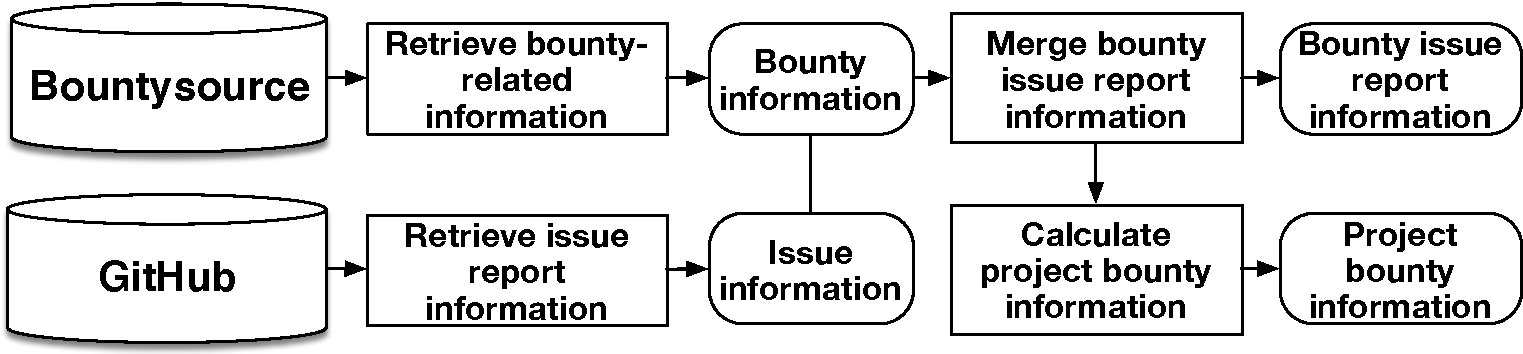
\includegraphics[width=9cm]{pics/datacollection/data_collection.pdf}
  \caption{An overview of our data collection process.}
  \label{overview}
  \vspace{-0.1in}

\end{figure}




All information about the bounties is stored on Bountysource and all details about issue reports and their corresponding projects are stored on GitHub. Hence, we collected data for our study along three dimensions: the bounty, the issue report, and the project.

\begin{figure}[t]
\centering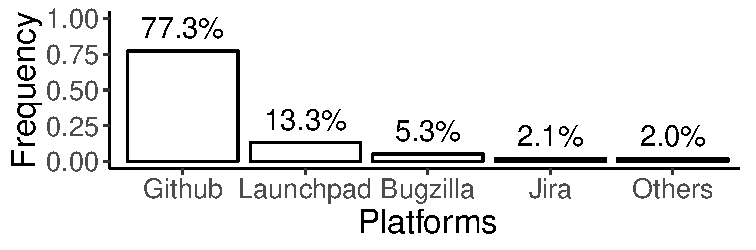
\includegraphics[width=0.8\columnwidth ]{pics/bg/RatioOfIssuesITS}
  \caption{The distribution of Bountysource bounties across the supported ITSs.}
  \label{RatioOfIssuesITS}
  \vspace{-0.1in}

\end{figure}

Figure~\ref{overview} presents an overview of our data collection process, which is broken down as follows:


\noindent\textbf{Step 1:} We retrieved the bounty and issue information from Bountysource using its official web API.\footnote{\url{https://bountysource.github.io/}} The bounty information includes the backers who proposed the bounty,  the proposed bounty value and the hunter who addressed the issue report. In addition, we collected basic information about the GitHub issue reports such as their id and URL.

\noindent\textbf{Step 2:} We retrieved the details of the issue reports, which are linked to Bountysource bounties by using the URL and id that we retrieved in step 1, from GitHub using its official web API.\footnote{\url{https://developer.github.com/v3/}} For example, we collected the description of the issue report, the creation date of the issue report, the comments that developers left under the issue, and the labels of the issue report.

\noindent\textbf{Step 3:} We calculated the corresponding project's bounty information for each collected bounty issue report, such as the number of total bounty issue reports of a project.



 \begin{table}[t]
   \centering
   \caption{Dataset description.}
     \begin{tabular}{p{24em}r}
    \hline
     Total number of bounties & 5,445 \bigstrut[t]\\
     Total number of claimed bounties & 2,402 \\
     Total bounty value & \$406,425 \\
     Total number of bounty hunters & 882 \\
     Total number of bounty backers & 2,534 \\
     Total number of issue reports & 3,509\\
     Total number of issue reports with multiple bounties & 795\\
     Total number of projects &  1,203 \bigstrut[b]\\
     \hline
     \end{tabular}%
   \label{tab:overviewOfGithub}%
   \vspace{-0.1in}

 \end{table}%


In total, we collected 5,445 bounties with a total value of \$406,425, together with their corresponding issue reports which were reported between Oct 19, 2012, and Oct 5, 2017. Table~\ref{tab:overviewOfGithub} gives a description of our dataset.


%We update the status of bounties for each issue at April 22, 2018 by Bountysource web-api\footnote{https://bountysource.github.io/}. \jy{Should introduce the distribution of issue-fixed day length to make the update reasonable?}

\begin{comment}
	
\begin{table}[ht]
  \centering
  \caption{Overview of the studied issues and their corresponding bounties. }
  \label{tab:overviewOfGithub}
  \begin{tabular}{|p{1cm}|p{1.6cm}|p{1.2cm}|p{1.2cm}|p{1.6cm}|p{1.3cm}|}
    \hline
    \textbf{\#Total Issue} & \textbf{\#Paid-out Issue} & \textbf{\#Total Bounty}& \textbf{\$Total Bounty}& \textbf{\$Paid-out Bounty}& \textbf{\#Bounty Hunter}\\
    \hline
   3,509&1,509  &5,445 &406,425 &218,824 &882  \\
    \hline
  \end{tabular}
\end{table}
\end{comment}




